%!TEX program = xelatex

\documentclass[a4paper, openany, oneside]{memoir}
\usepackage[no-math]{fontspec}
\usepackage{pgfplots}
\pgfplotsset{compat=newest}
\usepackage{commath}
\usepackage{mathtools}
\usepackage{amssymb}
\usepackage{amsthm}
\usepackage{booktabs}
\usepackage{mathtools}
\usepackage{xcolor}
\usepackage[separate-uncertainty=true, per-mode=symbol]{siunitx}
\usepackage[noabbrev, capitalize]{cleveref}
\usepackage{listings}
\usepackage[american inductor, european resistor]{circuitikz}
\usepackage{amsmath}
\usepackage{amsfonts}
\usepackage{ifxetex}
\usepackage[dutch,english]{babel}
\usepackage[backend=bibtexu,texencoding=utf8,bibencoding=utf8,style=ieee,sortlocale=en_GB,language=auto]{biblatex}
\usepackage[strict,autostyle]{csquotes}
\usepackage{parskip}
\usepackage{import}
\usepackage{standalone}
\usepackage{hyperref}
%\usepackage[toc,title,titletoc]{appendix}

\ifxetex{} % Fonts laden in het geval dat je met Xetex compiled
    \usepackage{fontspec}
    \defaultfontfeatures{Ligatures=TeX} % To support LaTeX quoting style
    \setromanfont{Palatino Linotype} % Tover ergens in Font mapje in root.
    \setmonofont{Source Code Pro}
\else % Terug val in standaard pdflatex tool chain. Geen ondersteuning voor OTT fonts
    \usepackage[T1]{fontenc}
    \usepackage[utf8]{inputenc}
\fi
\newcommand{\references}[1]{\begin{flushright}{#1}\end{flushright}}
\renewcommand{\vec}[1]{\boldsymbol{\mathbf{#1}}}
\newcommand{\uvec}[1]{\boldsymbol{\hat{\vec{#1}}}}
\newcommand{\mat}[1]{\boldsymbol{\mathbf{#1}}}
\newcommand{\fasor}[1]{\boldsymbol{\tilde{\vec{#1}}}}
\newcommand{\cmplx}[0]{\mathrm{j}}
\renewcommand{\Re}[0]{\operatorname{Re}}
\newcommand{\Cov}{\operatorname{Cov}}
\newcommand{\Var}{\operatorname{Var}}
\newcommand{\proj}{\operatorname{proj}}
\newcommand{\Perp}{\operatorname{perp}}
\newcommand{\col}{\operatorname{col}}
\newcommand{\rect}{\operatorname{rect}}
\newcommand{\sinc}{\operatorname{sinc}}
\newcommand{\IT}{\operatorname{IT}}
\newcommand{\F}{\mathcal{F}}

\newtheorem{definition}{Definition}
\newtheorem{theorem}{Theorem}


\DeclareSIUnit{\voltampere}{VA} %apparent power
\DeclareSIUnit{\pii}{\ensuremath{\pi}}

\hypersetup{%setup hyperlinks
    colorlinks,
    citecolor=black,
    filecolor=black,
    linkcolor=black,
    urlcolor=black
}

% Example boxes
\usepackage{fancybox}
\usepackage{framed}
\usepackage{adjustbox}
\newenvironment{simpages}%
{\AtBeginEnvironment{itemize}{\parskip=0pt\parsep=0pt\partopsep=0pt}
\def\FrameCommand{\fboxsep=.5\FrameSep\shadowbox}\MakeFramed{\FrameRestore}}%
{\endMakeFramed}

% Impulse train
\DeclareFontFamily{U}{wncy}{}
\DeclareFontShape{U}{wncy}{m}{n}{<->wncyr10}{}
\DeclareSymbolFont{mcy}{U}{wncy}{m}{n}
\DeclareMathSymbol{\Sha}{\mathord}{mcy}{"58}
\addbibresource{../../../includes/bibliography.bib}

\title{Compressive Sensing - An Overview}

\author{W.P. Bruinsma \and R.P. Hes \and H.J.C. Kroep \and T.C. Leliveld \and W.M. Melching \and T.A. aan de Wiel}

\raggedbottom

\begin{document}
\section{Call graphs source}
\label{sec:call_graphs_source}
\subsection{Sinusoidal}
\label{sub:sinusoidal}
\begin{figure}[H]
    \centering
    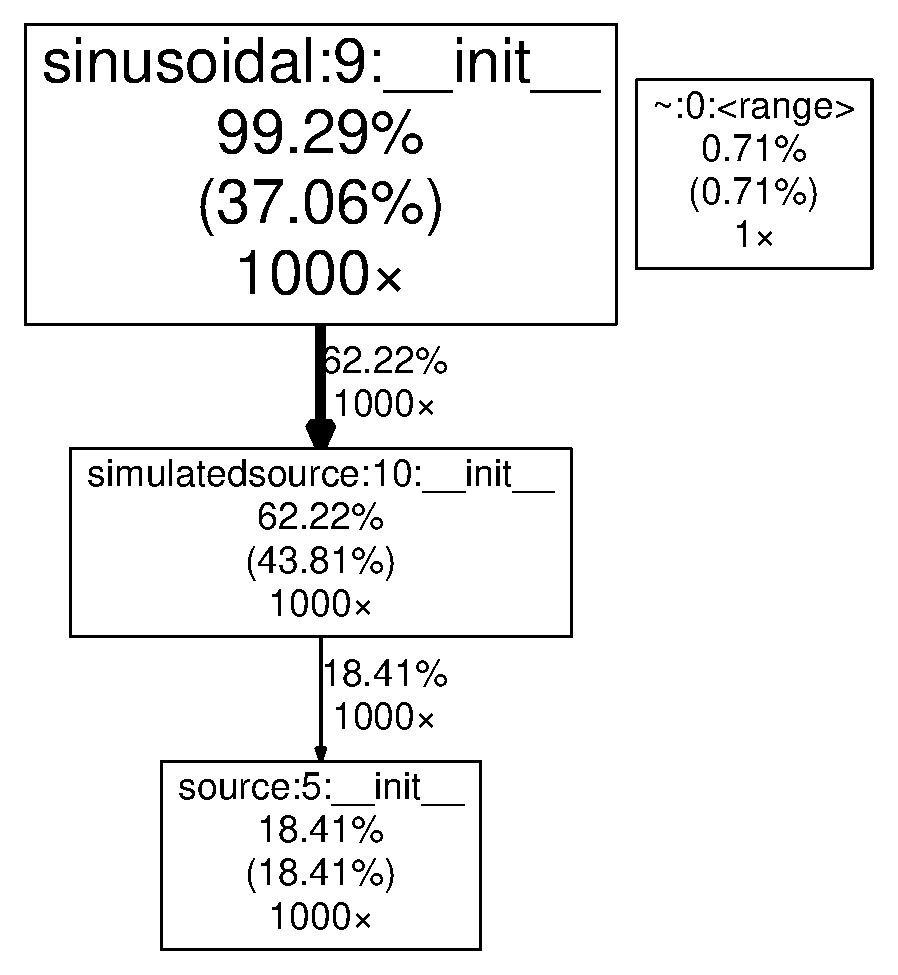
\includegraphics[width=0.8\linewidth]{Sinusoidal_init}
    \caption{Sinusoidal\_init call graph}
    \label{fig:Sinusoidal_init}
\end{figure}

\begin{figure}[H]
    \centering
    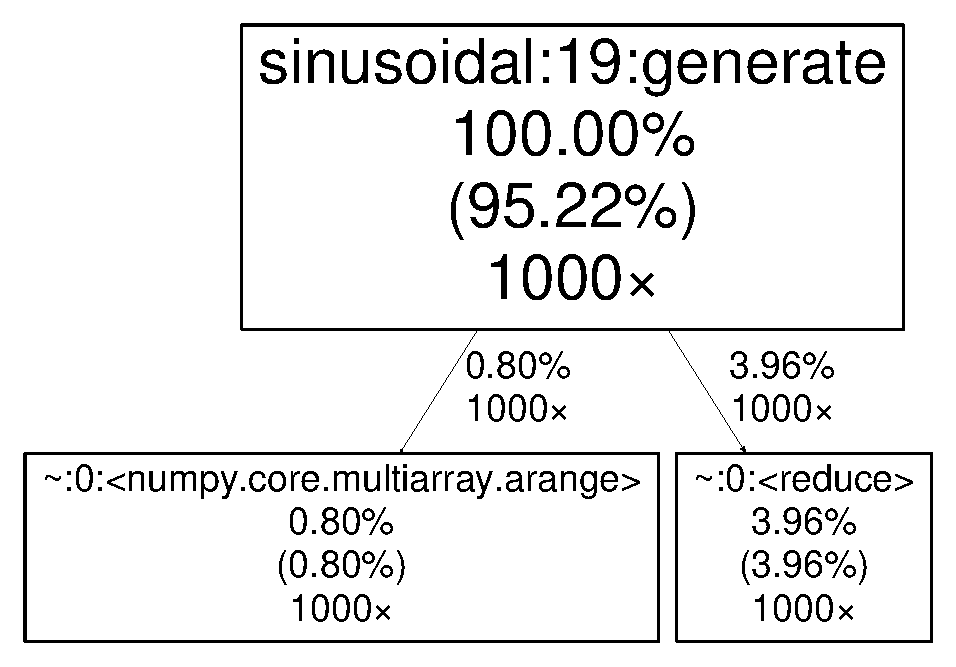
\includegraphics[width=0.8\linewidth]{Sinusoidal_generate}
    \caption{Sinusoidal\_generate call graph}
    \label{fig:Sinusoidal_generate}
\end{figure}

\subsection{Complex exponential}
\label{sub:complex_exponential}

\begin{figure}[H]
    \centering
    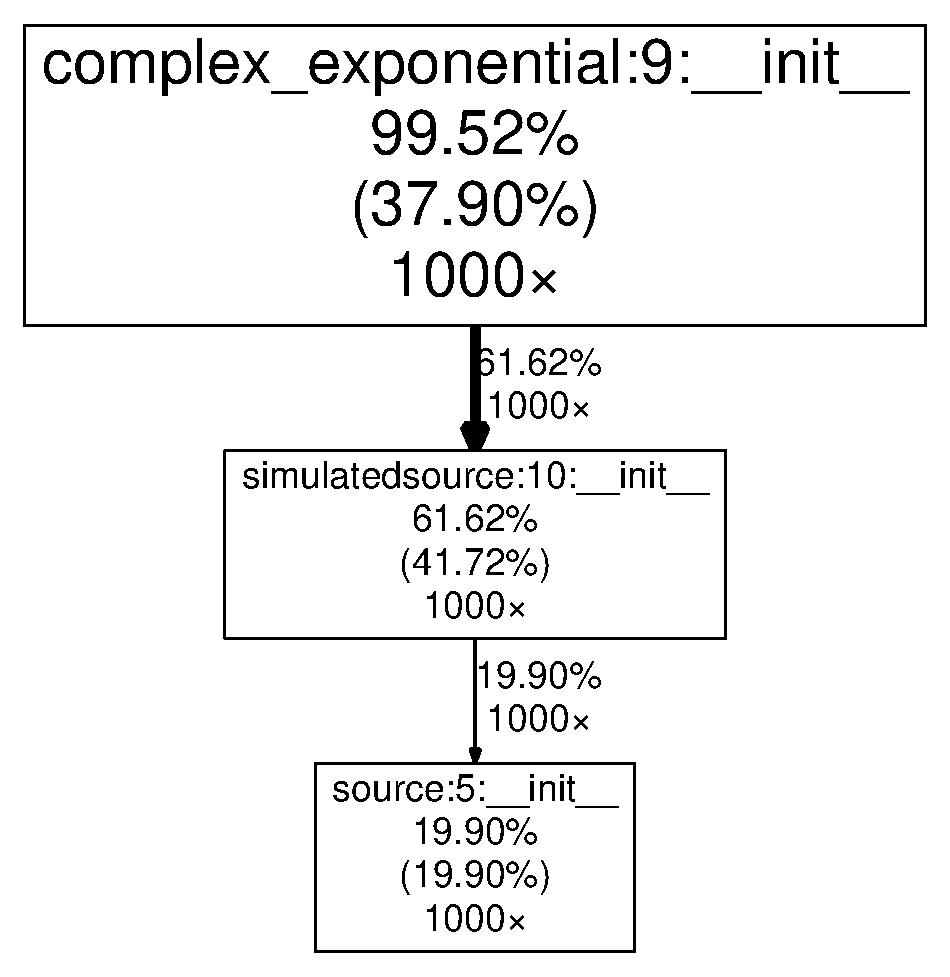
\includegraphics[width=0.8\linewidth]{ComplexExponential_init}
    \caption{ComplexExponential\_init call graph.}
    \label{fig:ComplexExponential_init}
\end{figure}

\begin{figure}[H]
    \centering
    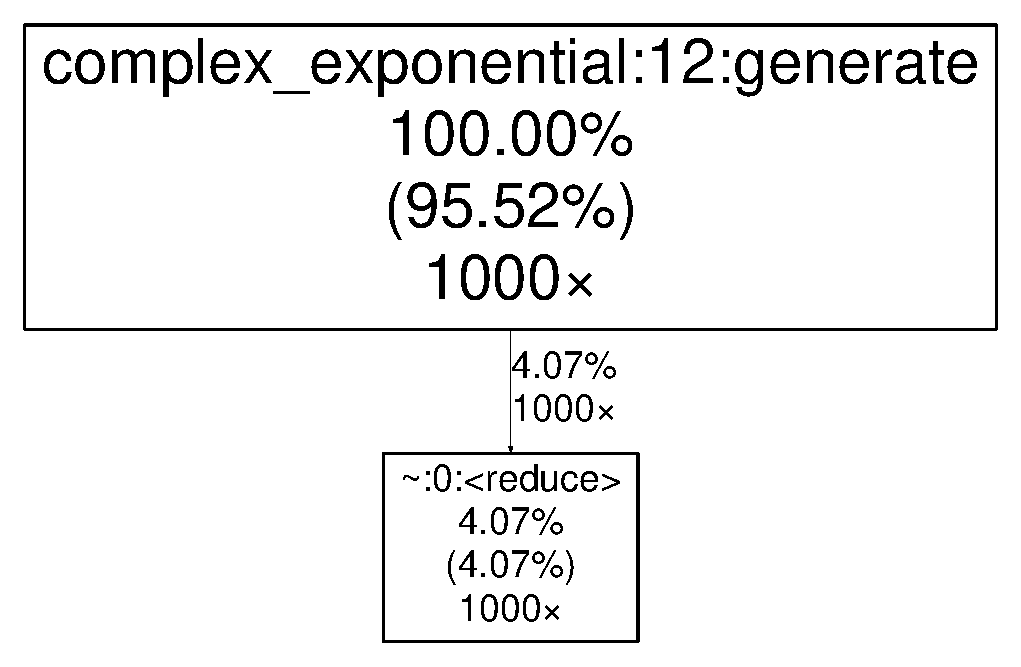
\includegraphics[width=0.8\linewidth]{ComplexExponential_generate}
    \caption{ComplexExponential\_generate call graph}
    \label{fig:ComplexExponential_generate}
\end{figure}

\subsection{Rectangular source}
\label{sub:rectangular_source}

\begin{figure}[H]
    \centering
    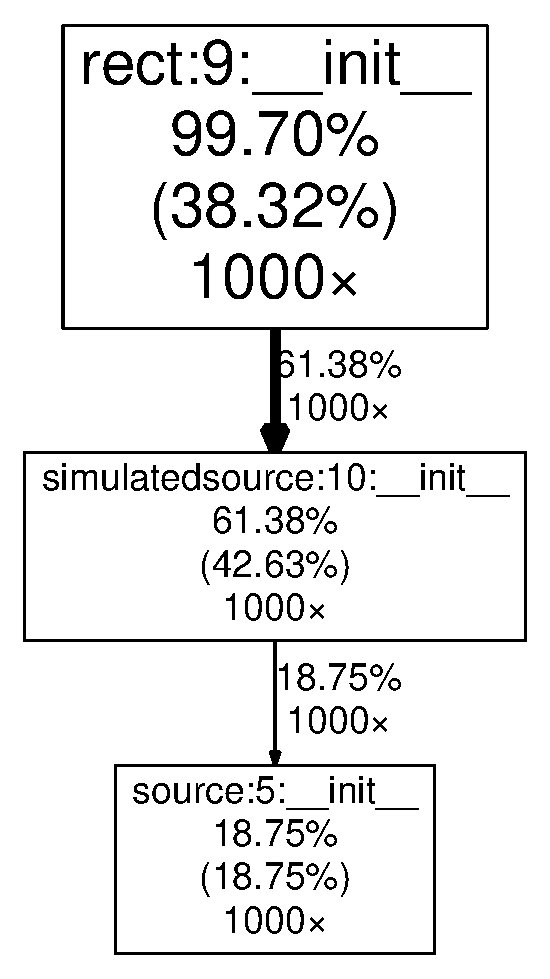
\includegraphics[width=0.8\linewidth]{Rect_init}
    \caption{Rect\_init call graph.}
    \label{fig:Rect_init}
\end{figure}

\begin{figure}[H]
    \centering
    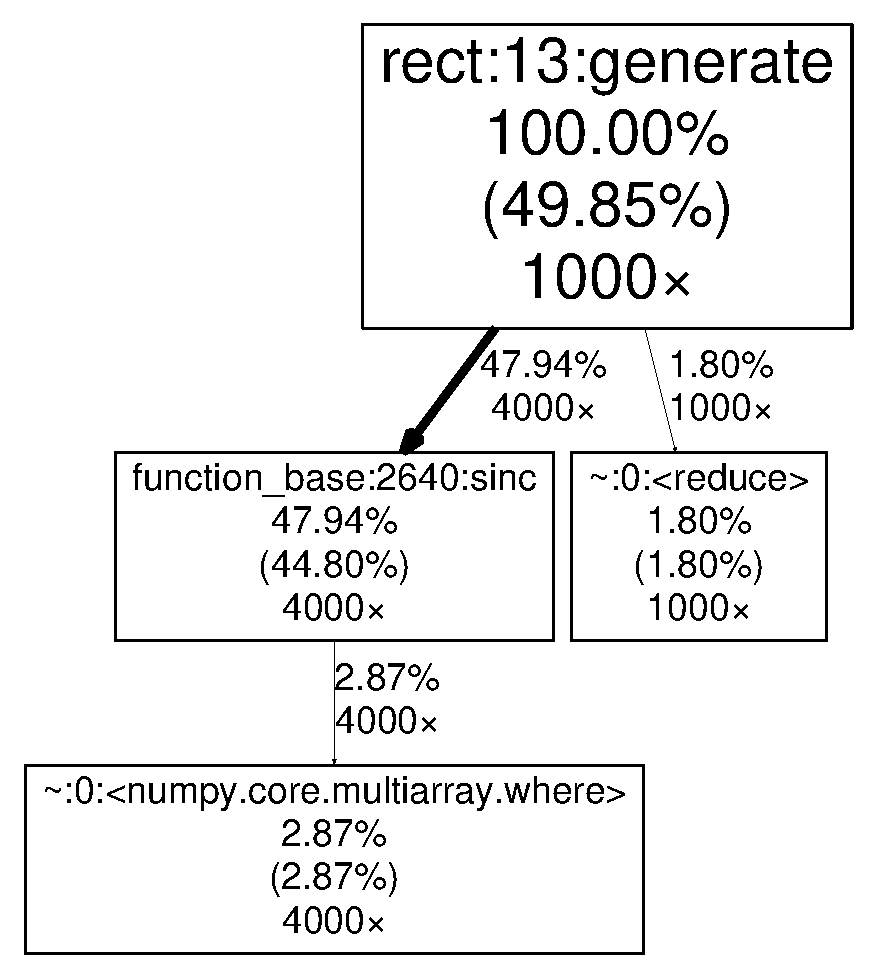
\includegraphics[width=0.8\linewidth]{Rect_generate}
    \caption{Rect\_generate call graph}
    \label{fig:Rect_generate}
\end{figure}

\section{Sampling call graphs}
\label{sec:sampling_call_graphs}
\subsection{Multicoset sampler}
\label{sub:multicoset_sampler}

\begin{figure}[H]
    \centering
    \includegraphics[width=0.8\linewidth]{Multicoset_init}
    \caption{Multicoset\_init call graph}
    \label{fig:Multicoset_init}
\end{figure}

\begin{figure}[H]
    \centering
    \includegraphics[width=0.8\linewidth]{Multicoset_sample}
    \caption{Multicoset\_sample call graph}
    \label{fig:Multicoset_sample}
\end{figure}

\subsection{Coprime sampler}
\label{sub:coprime_sampler}

\begin{figure}[H]
    \centering
    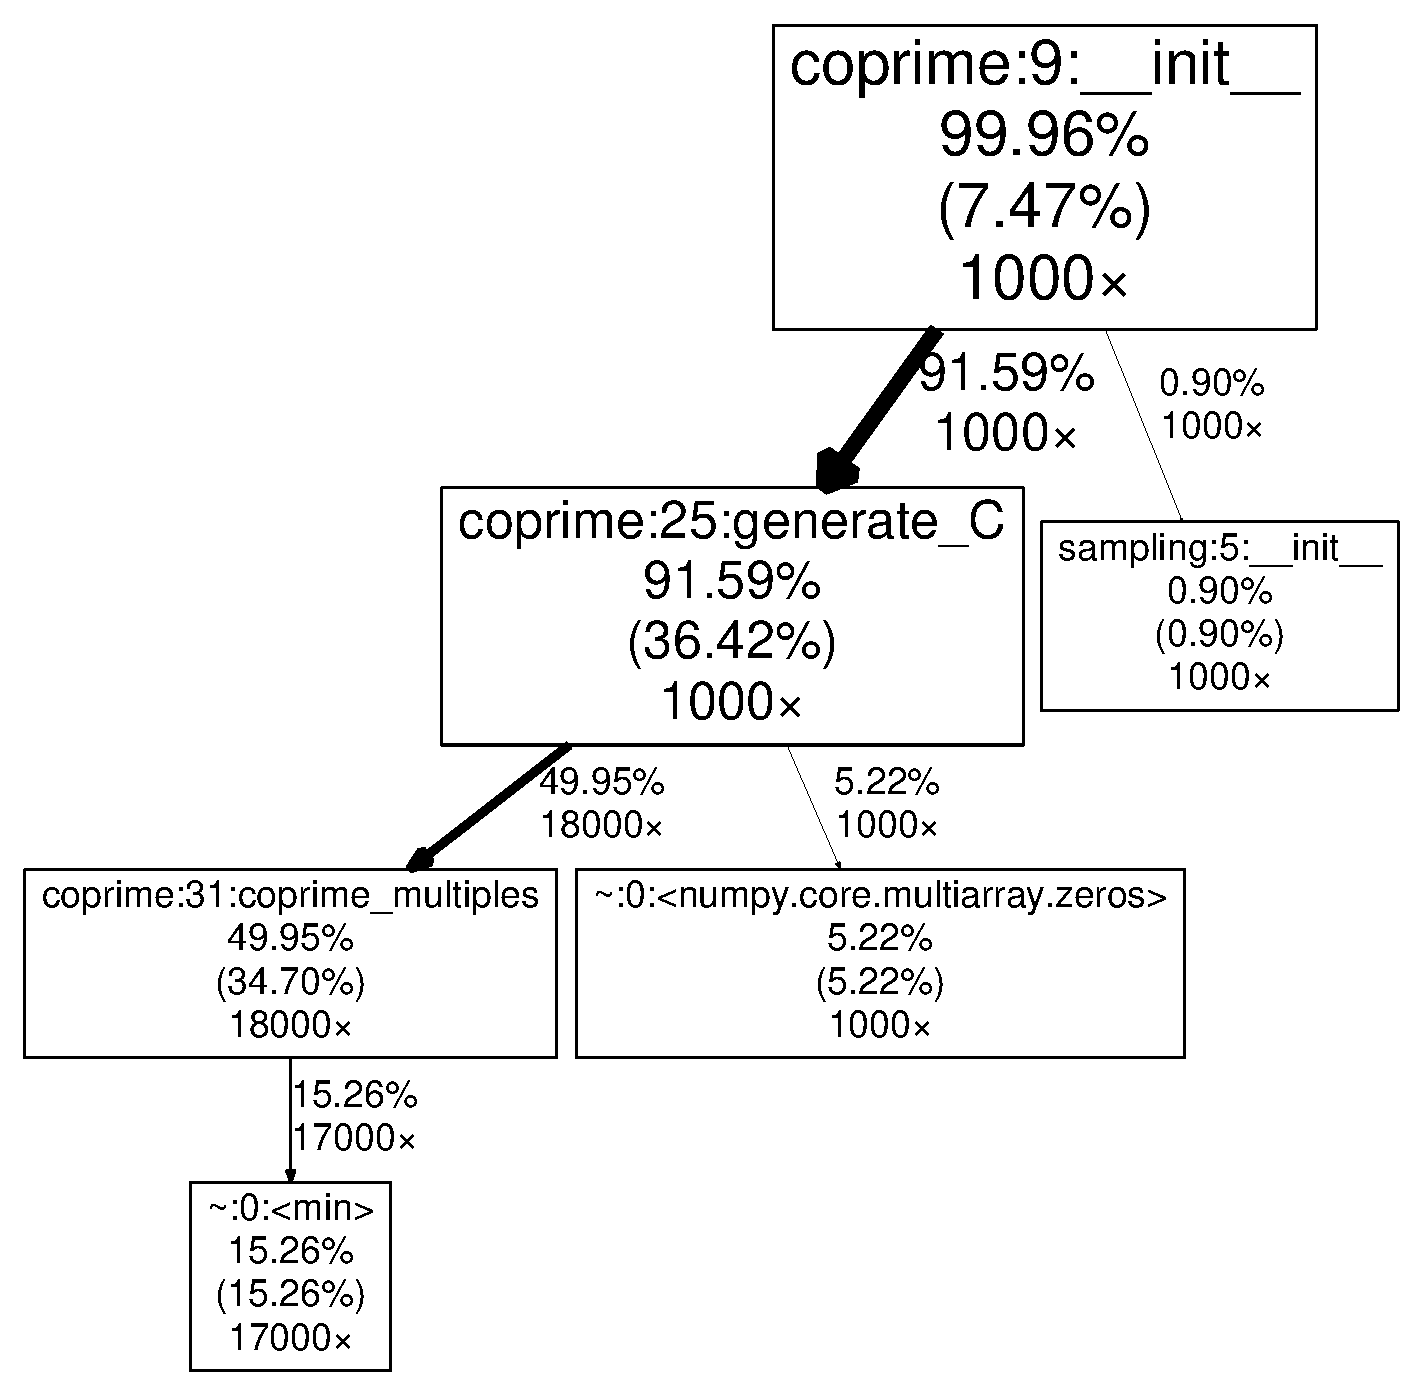
\includegraphics[width=0.8\linewidth]{Coprime_init}
    \caption{Coprime\_init call graph.}
    \label{fig:Coprime_init}
\end{figure}

\begin{figure}[H]
    \centering
    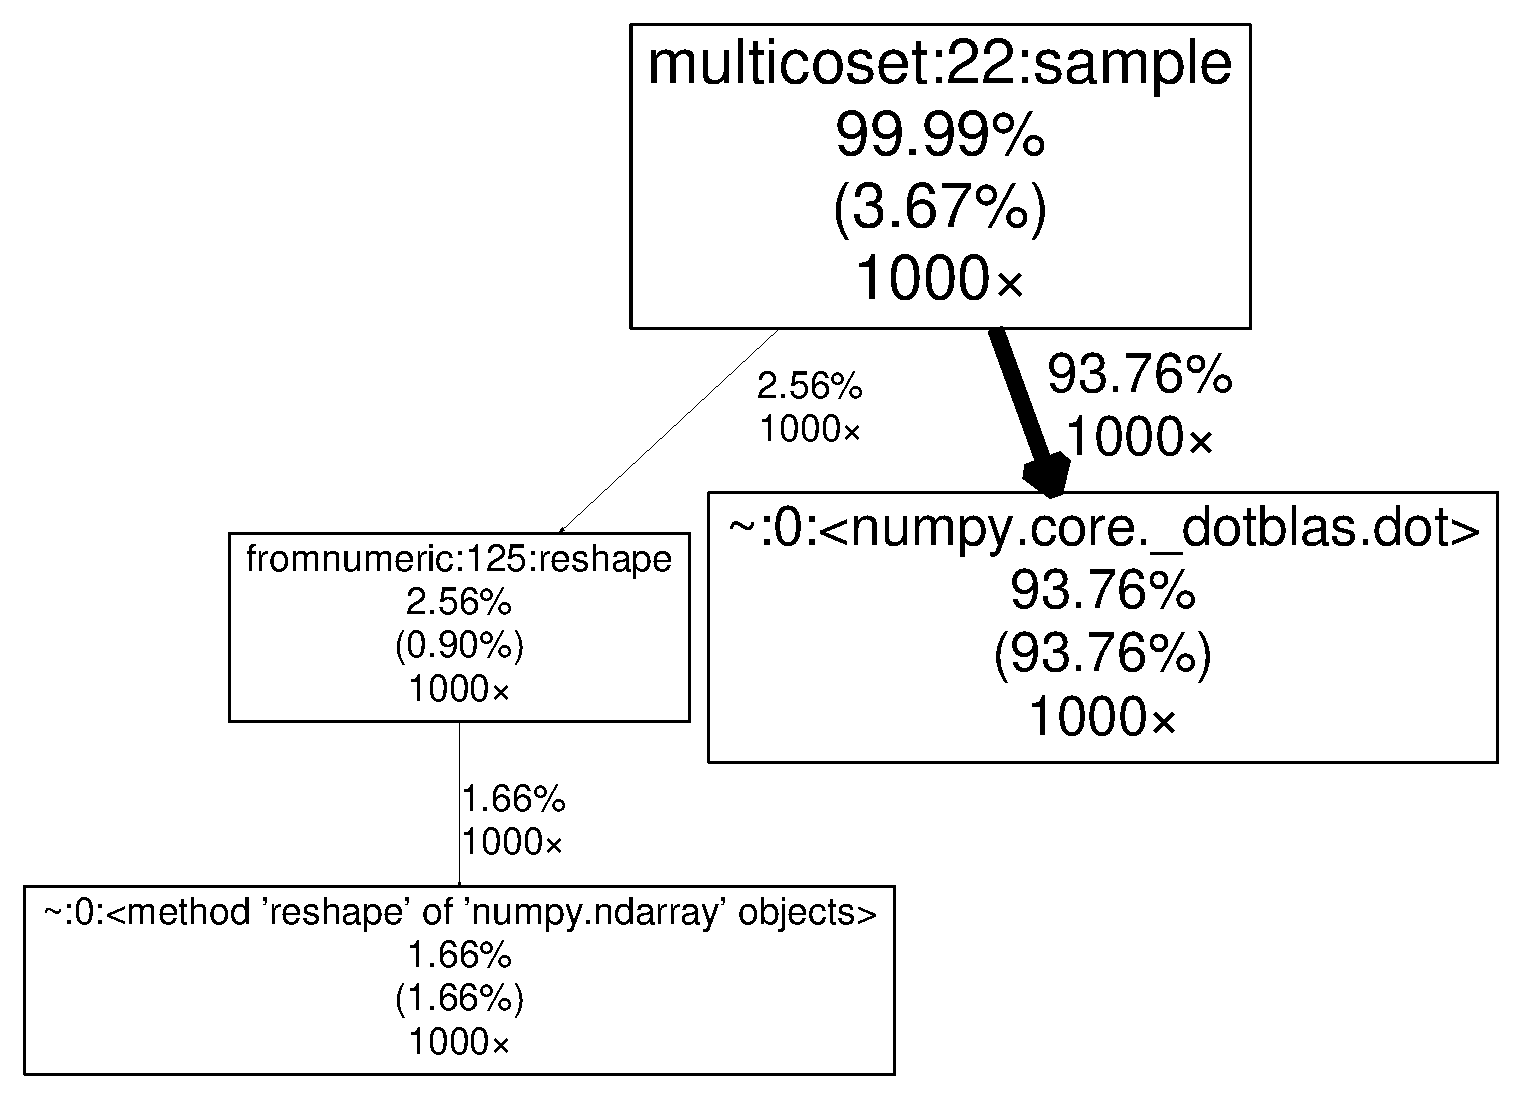
\includegraphics[width=0.8\linewidth]{Coprime_sample}
    \caption{Coprime\_sample call graph.}
    \label{fig:Coprime_sample}
\end{figure}

\section{Reconstructor call graphs}
\label{sec:reconstructor_call_graphs}

\begin{figure}[H]
    \centering
    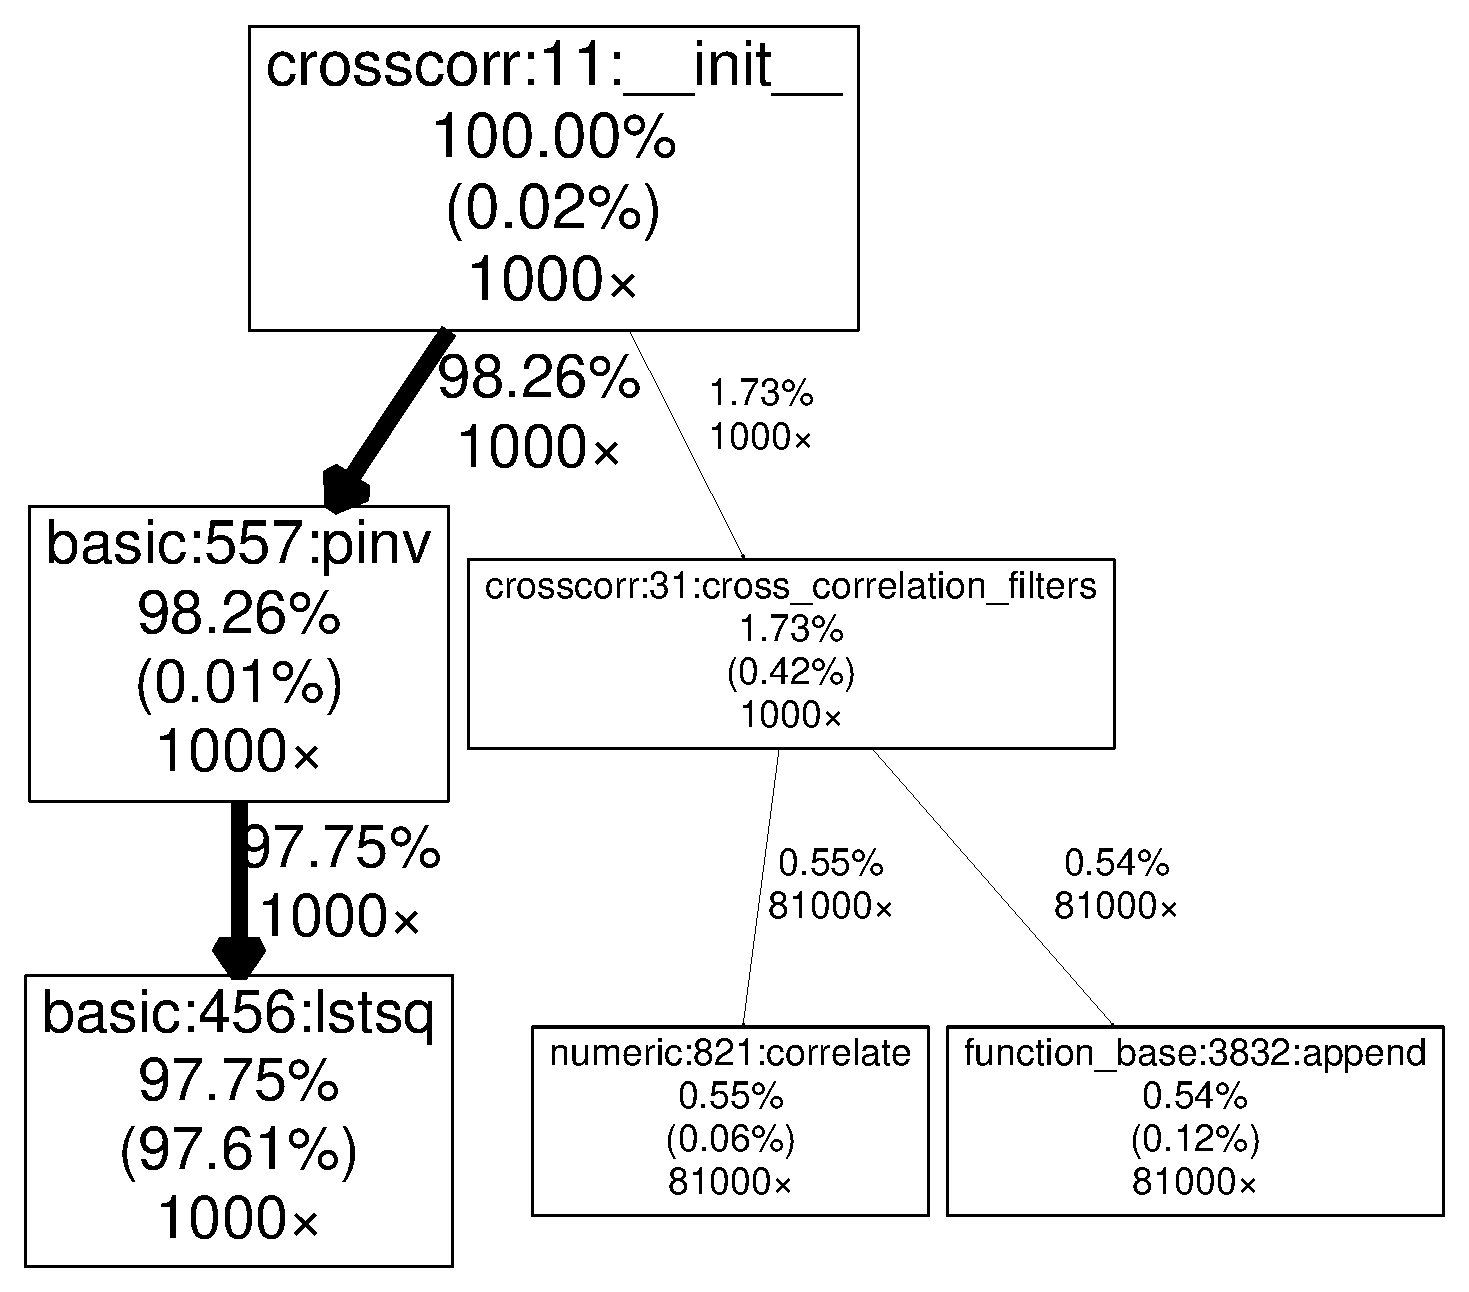
\includegraphics[width=0.8\linewidth]{CrossCorrelation_init}
    \caption{CrossCorrelation\_init call graph.}
    \label{fig:CrossCorrelation_init}
\end{figure}

\begin{figure}[H]
    \centering
    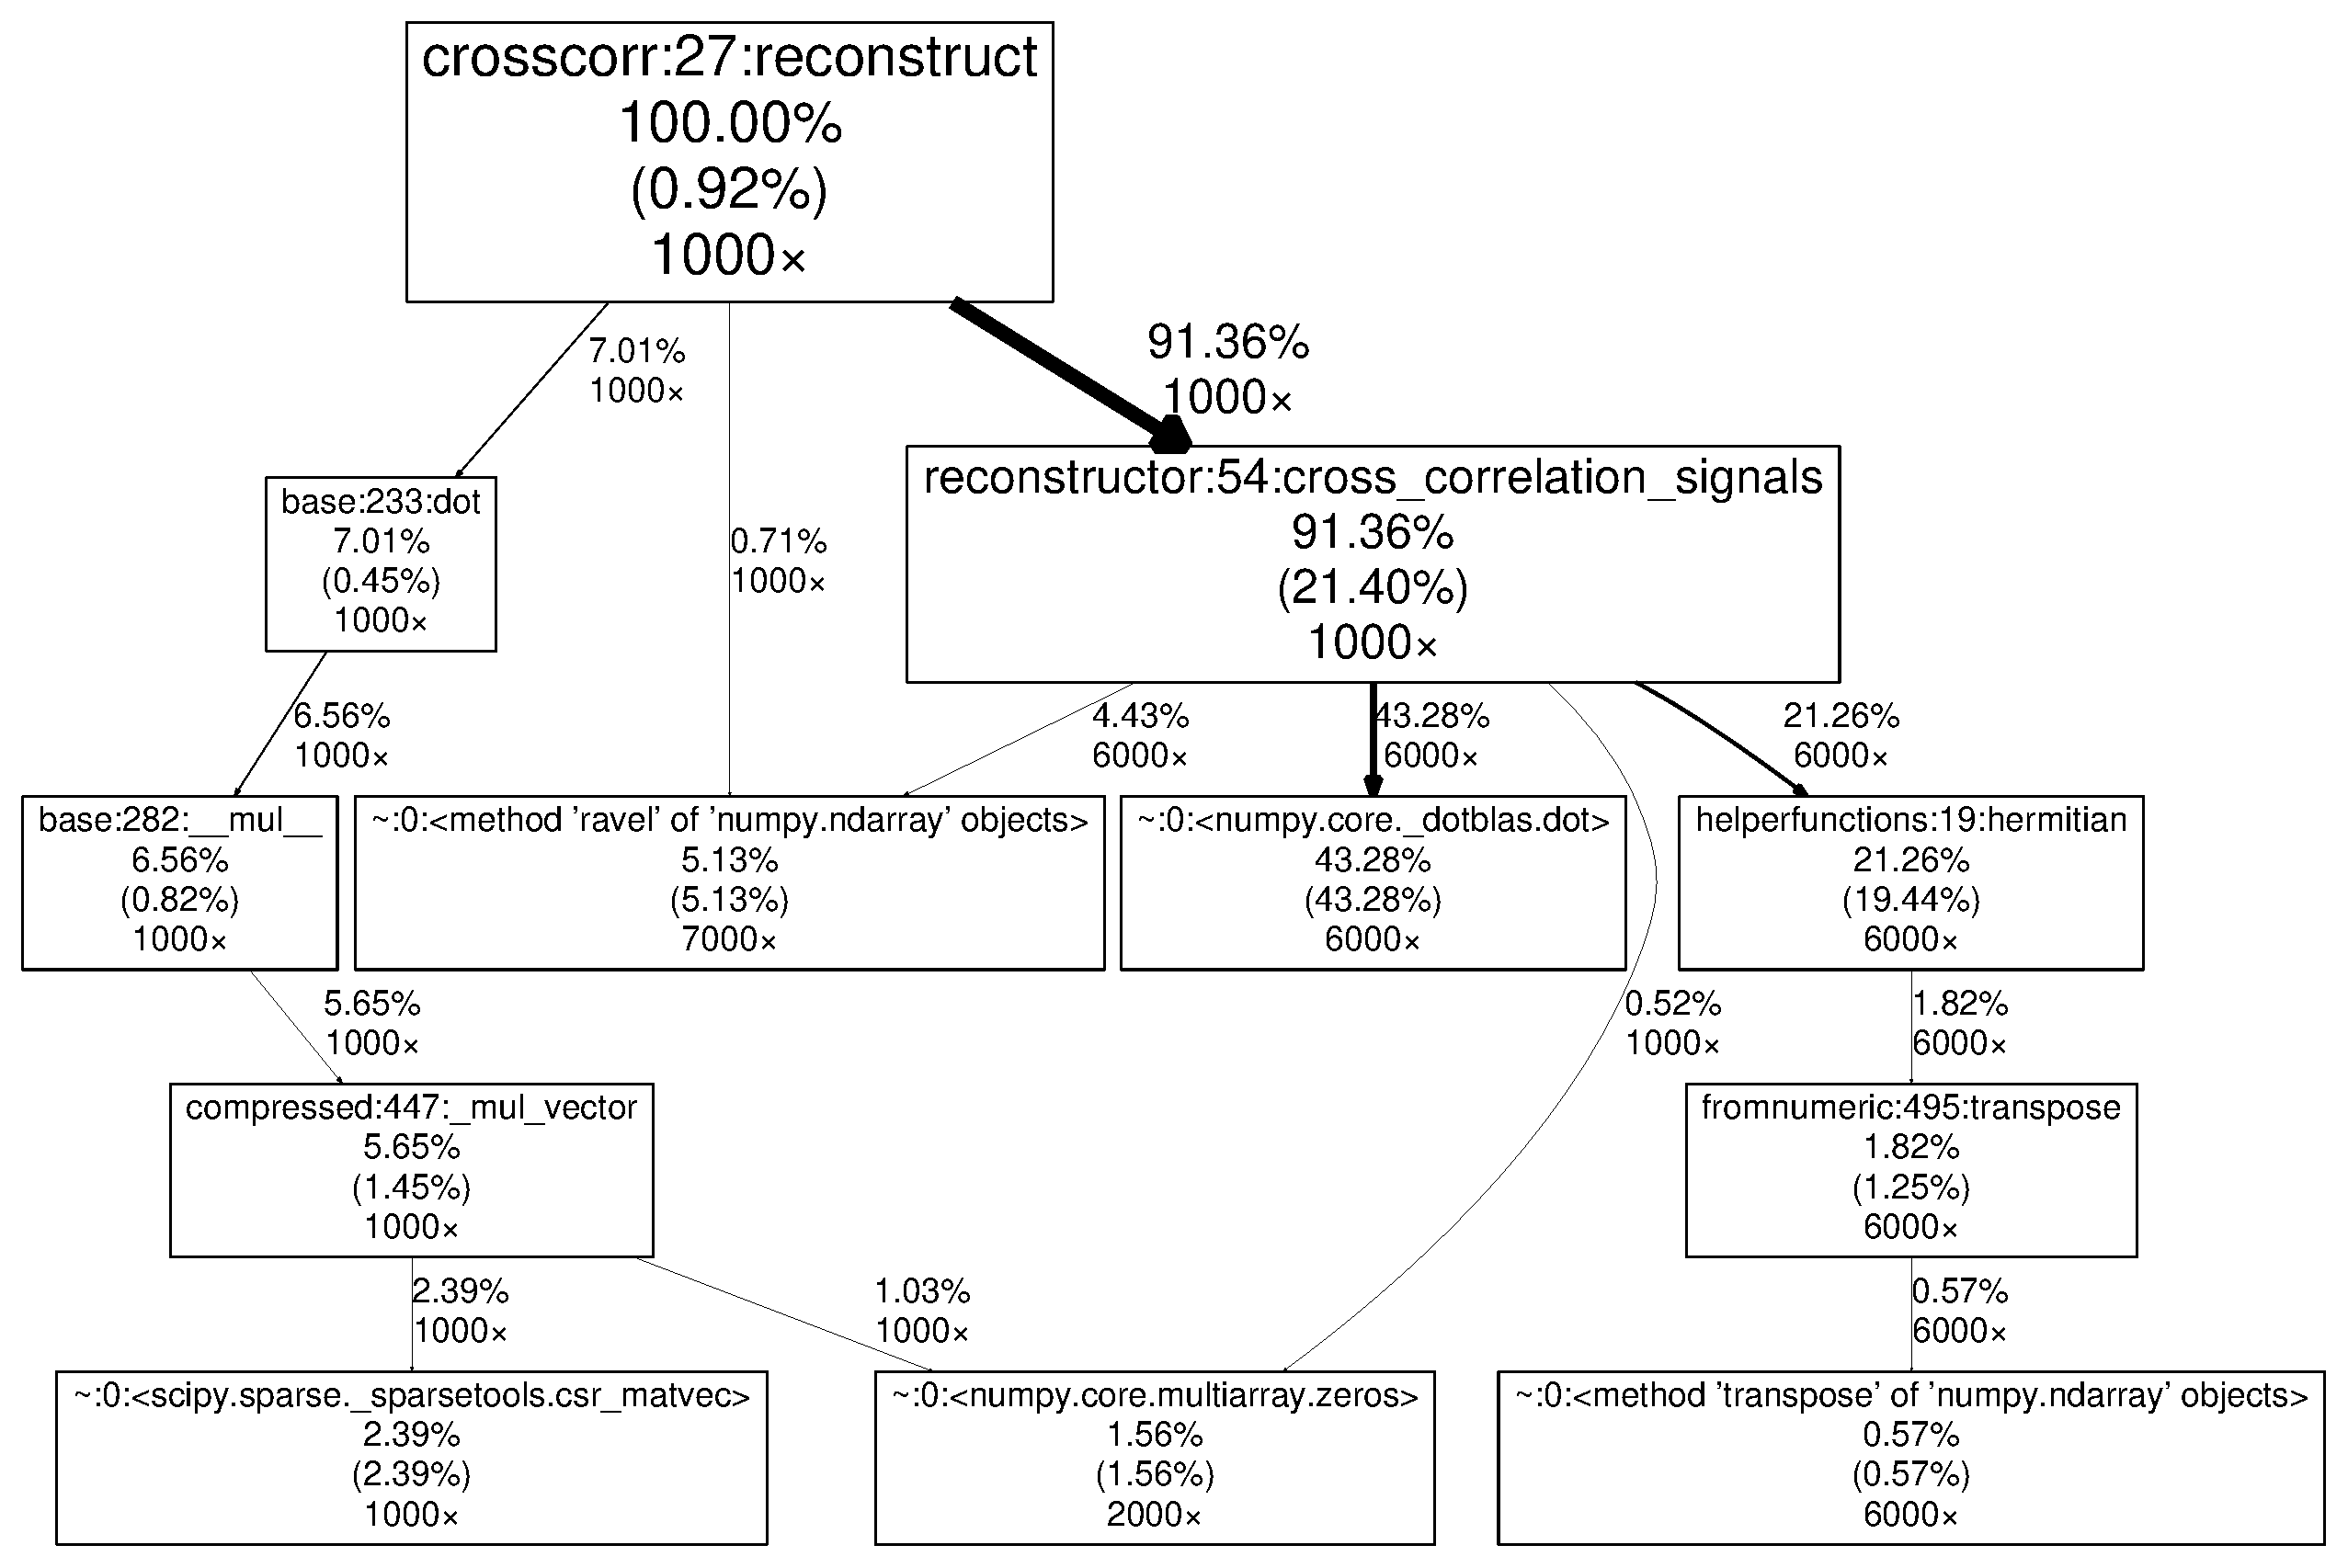
\includegraphics[width=0.8\linewidth]{CrossCorrelation_reconstruct}
    \caption{CrossCorrelation\_reconstruct call graph.}
    \label{fig:CrossCorrelation_reconstruct}
\end{figure}

\subsection{Wessel}
\label{sub:wessel}

\begin{figure}[H]
    \centering
    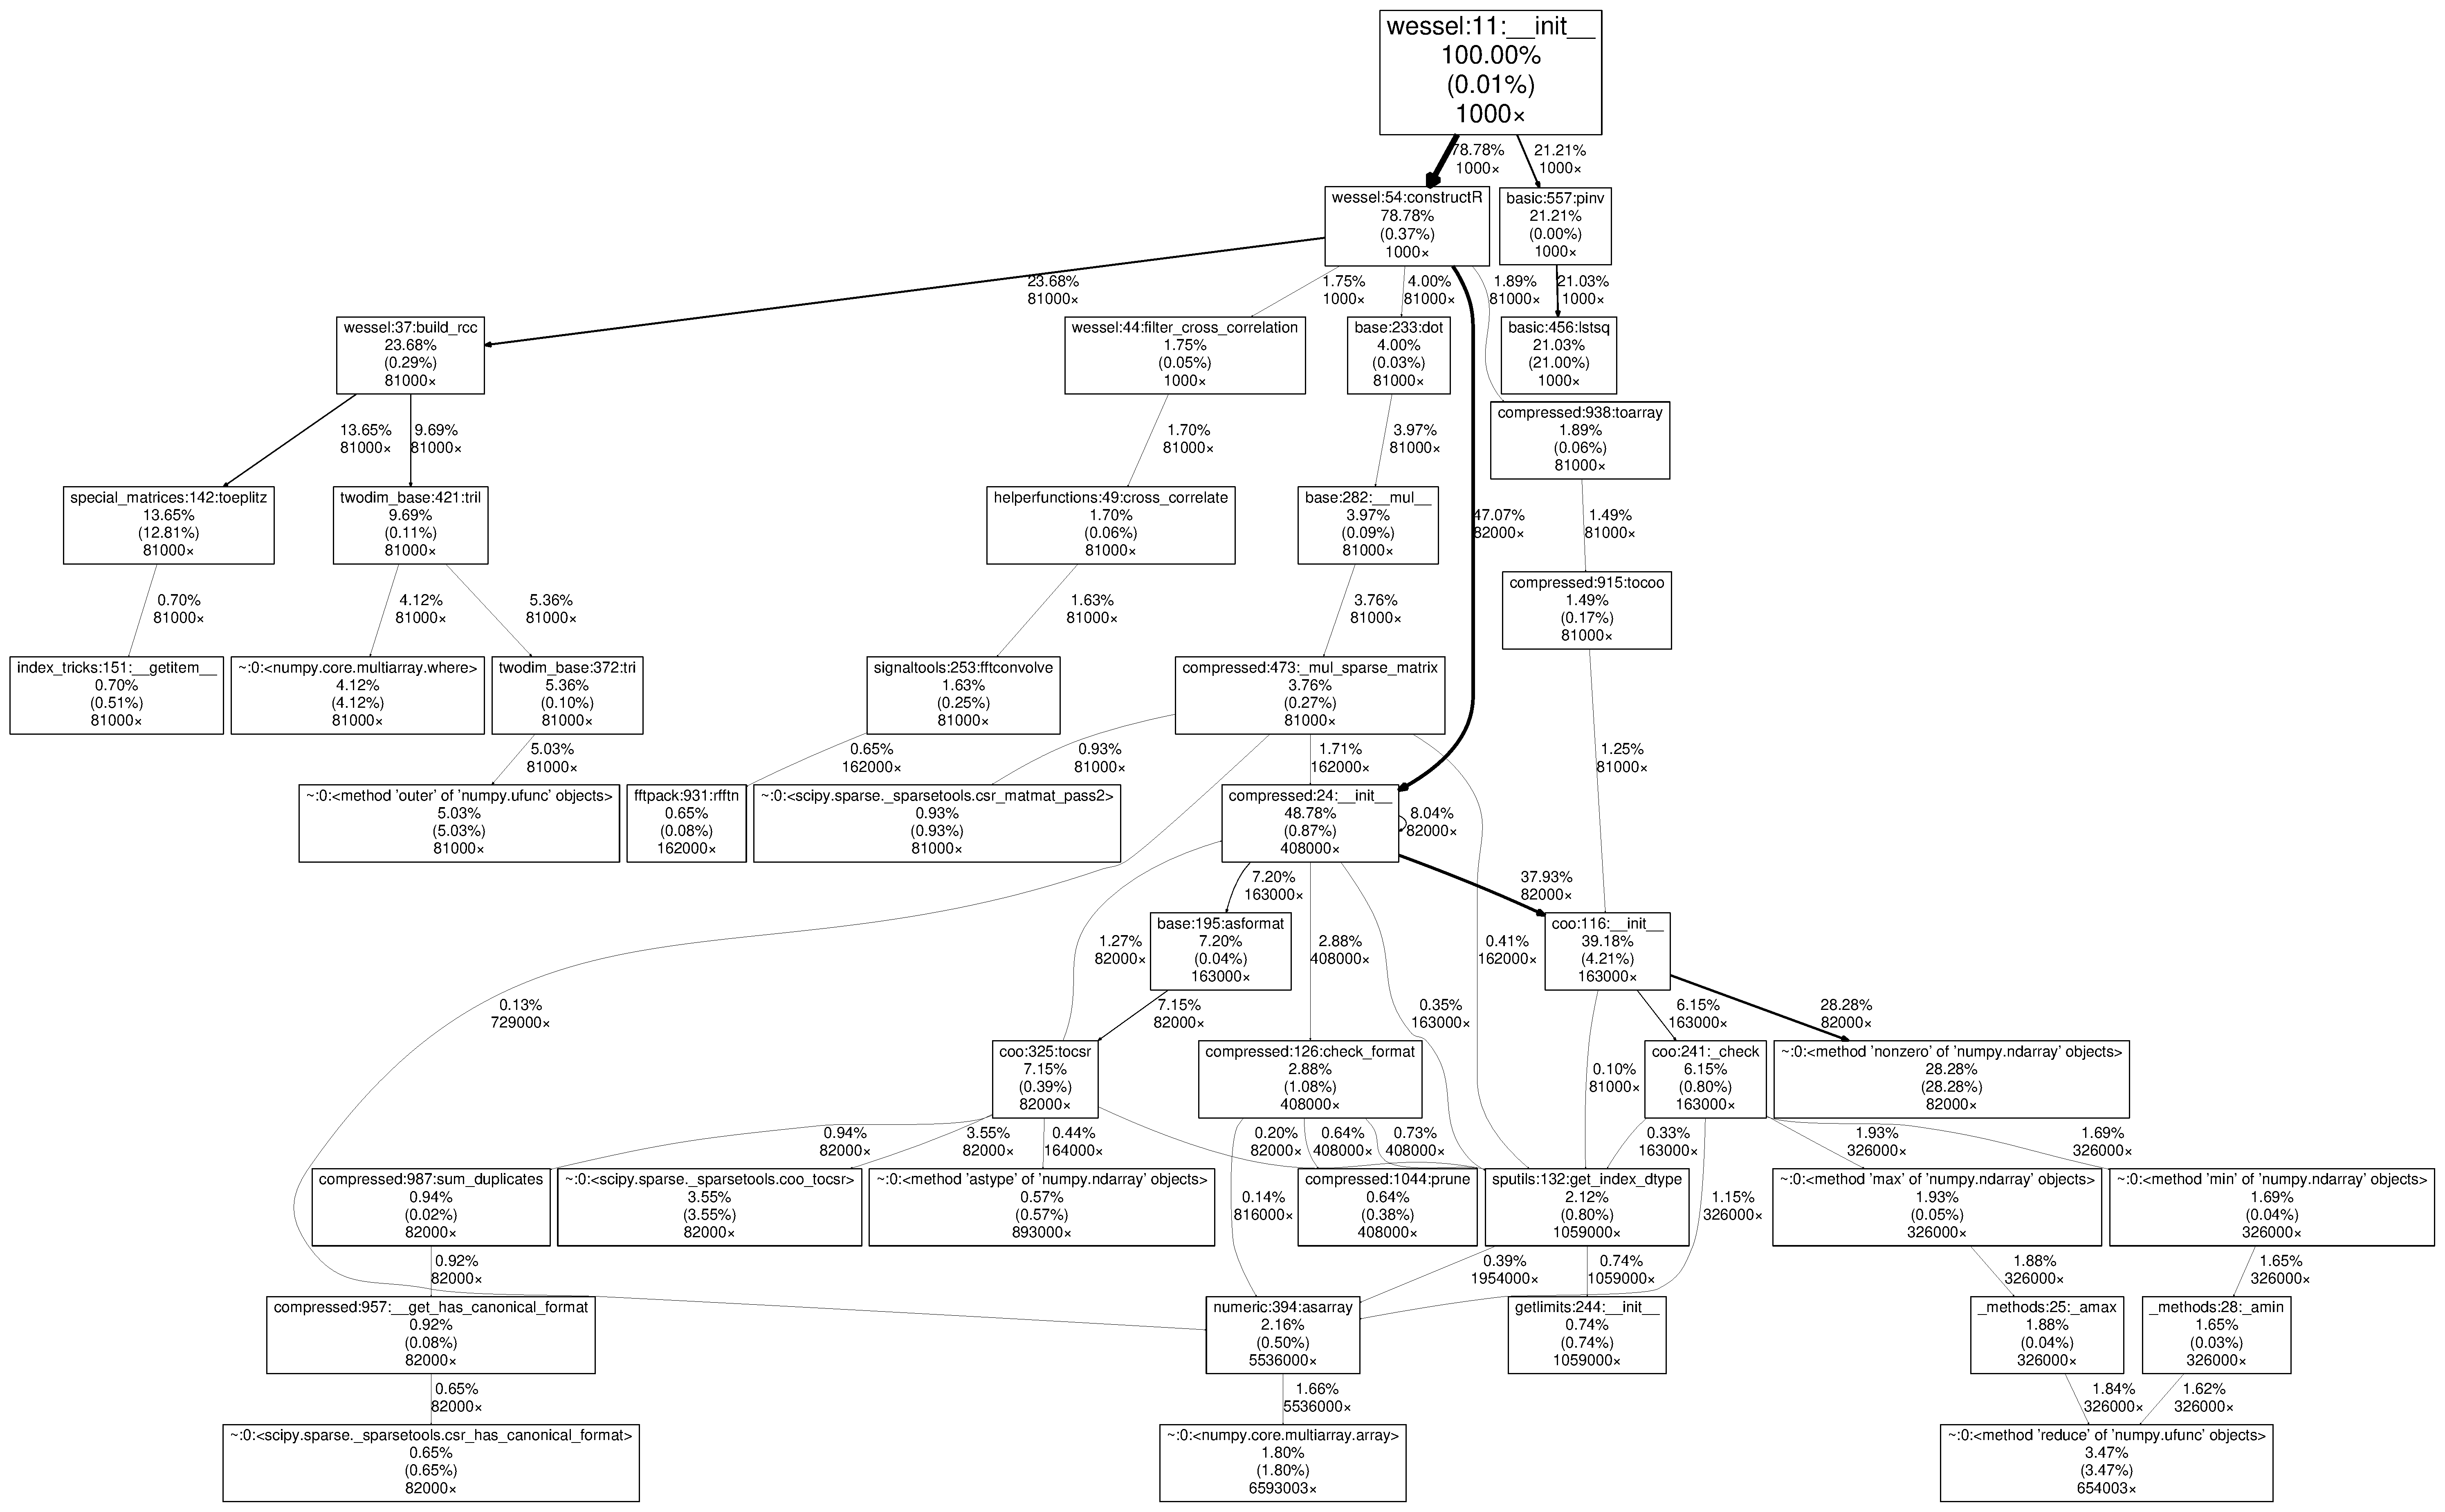
\includegraphics[width=0.8\linewidth]{Wessel_init}
    \caption{Wessel\_init call graph.}
    \label{fig:Wessel_init}
\end{figure}

\begin{figure}[H]
    \centering
    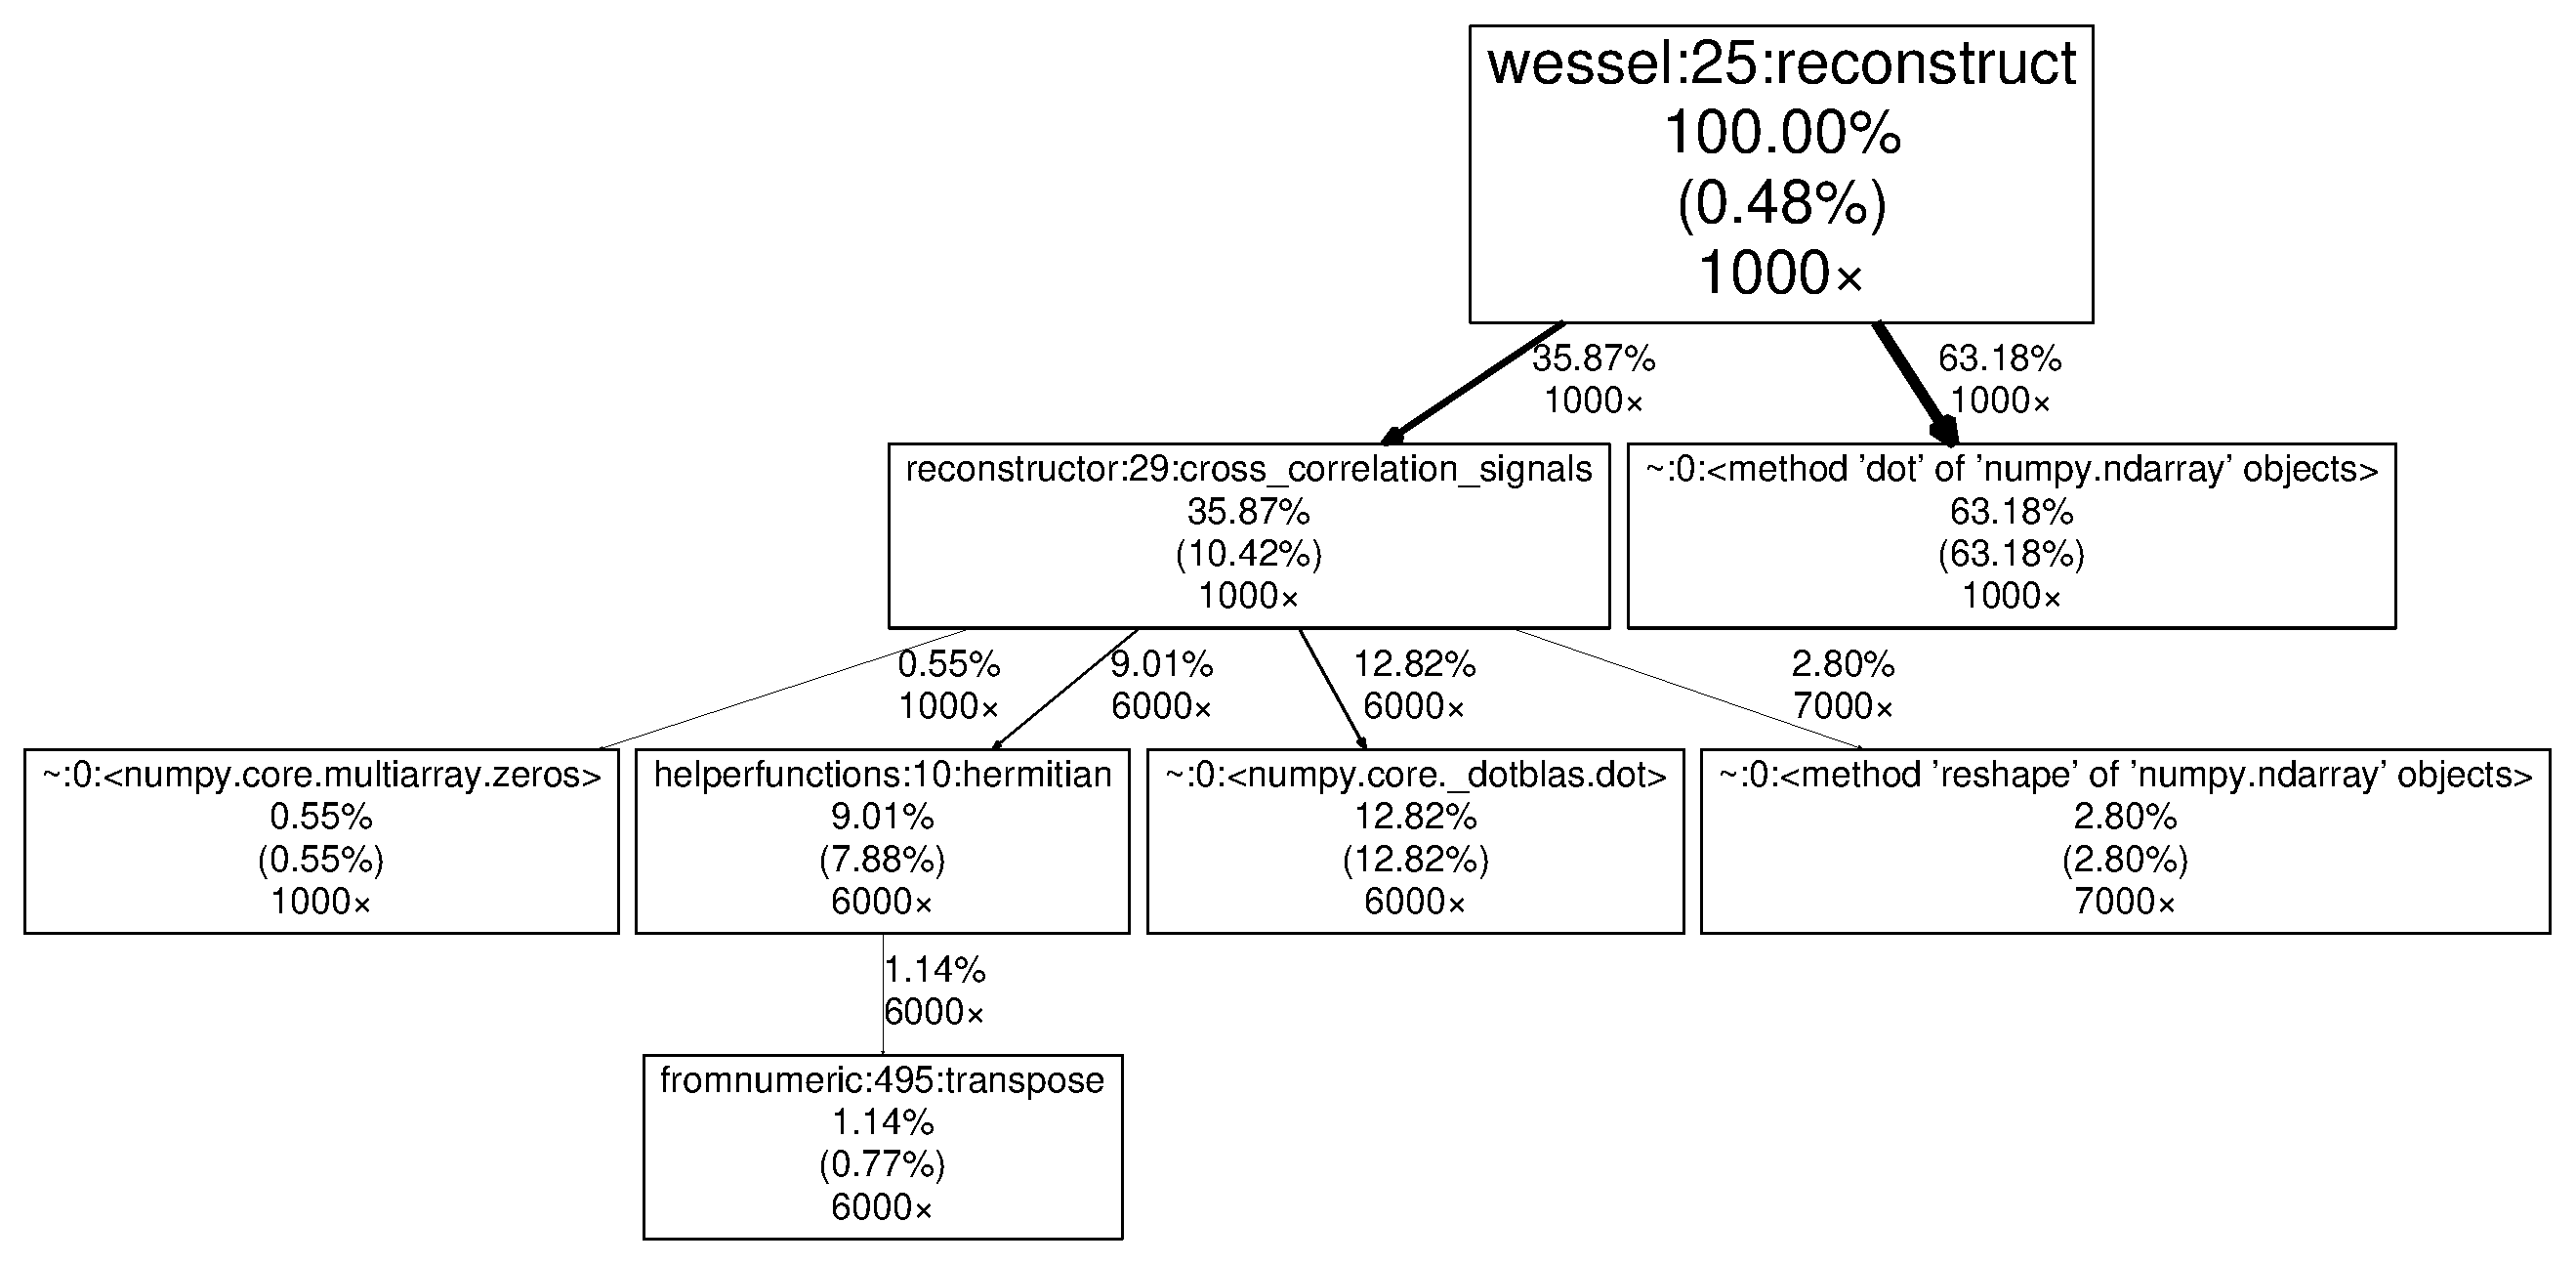
\includegraphics[width=0.8\linewidth]{Wessel_reconstruct}
    \caption{Wessel\_reconstruct call graph.}
    \label{fig:Wessel_reconstruct}
\end{figure}










\end{document}
